\documentclass{article}

% if you need to pass options to natbib, use, e.g.:
% \PassOptionsToPackage{numbers, compress}{natbib}
% before loading nips_2017
%
% to avoid loading the natbib package, add option nonatbib:
% \usepackage[nonatbib]{nips_2017}

\usepackage[final]{nips_2017}

\usepackage{graphicx}
\usepackage[utf8]{inputenc} % allow utf-8 input
\usepackage[T1]{fontenc}    % use 8-bit T1 fonts
\usepackage{hyperref}       % hyperlinks
\usepackage{url}            % simple URL typesetting
\usepackage{booktabs}       % professional-quality tables
\usepackage{amsfonts}       % blackboard math symbols
\usepackage{nicefrac}       % compact symbols for 1/2, etc.
\usepackage{microtype}      % microtypography

% Choose a title for your submission
\title{Your title here}


\author{Student 1 \qquad Student 2 \qquad Student 3}

\begin{document}
% \nipsfinalcopy is no longer used

\maketitle

% We do not requrire you to write an abstract. Still, if you feel like it, please do so.
%\begin{abstract}
%\end{abstract}

Feel free to add more sections but those listed here are strongly recommended.
\section{Introduction}
Natural language is
You can keep this short. Ideally you introduce the task already in a way that highlights the difficulties  your method will tackle.
\section{Methodology}
The idea of our approach follows that of successes in previous work such as \cite{UWNLP} and \cite{COGCOMP}. More specifically our approach consists of training a binary logistic regression classifier based on an augmented data set which we create ourselves. This augmentation is based on ideas that have been successfully used in the past (e.g. \cite{LSTMClassifier}). As features for our classifier we consider a collection of feature extractors which produce a vector of features for any 5 sentence story.

\subsection{Data augmentation}
The augmented data set is composed of labeled 5 sentence stories. We create it by combining the original data set and a negative data set. Here the original dataset gets assigned a positive label and the negative set a negative label. We compose the negative dataset by replacing the ending of each 5 sentence story by a randomly selected ending, as done by \cite{LSTMClassifier}. We use a replication factor of 1, i.e. for every sample of the original training set we add a single negative sample.

\subsection{Feature extraction}
In order to fit a logistic regression model as described above we use features obtained from feature extractors. A feature extractor is simply a model which takes in a 5 sentence story and outputs a feature or vector of features. Feature extractors are discussed extensively in section 3. To obtain the final set of features we simply combine features from all extractors for each sample.
%Your idea. You can rename this section if you like. Early on in this section -- but not necessarily first -- make clear what category your method falls into: Is it generative? Discriminative? Is there a particular additional data source you want to use?

\section{Model}

	\begin{figure}[h!]
		\centering
		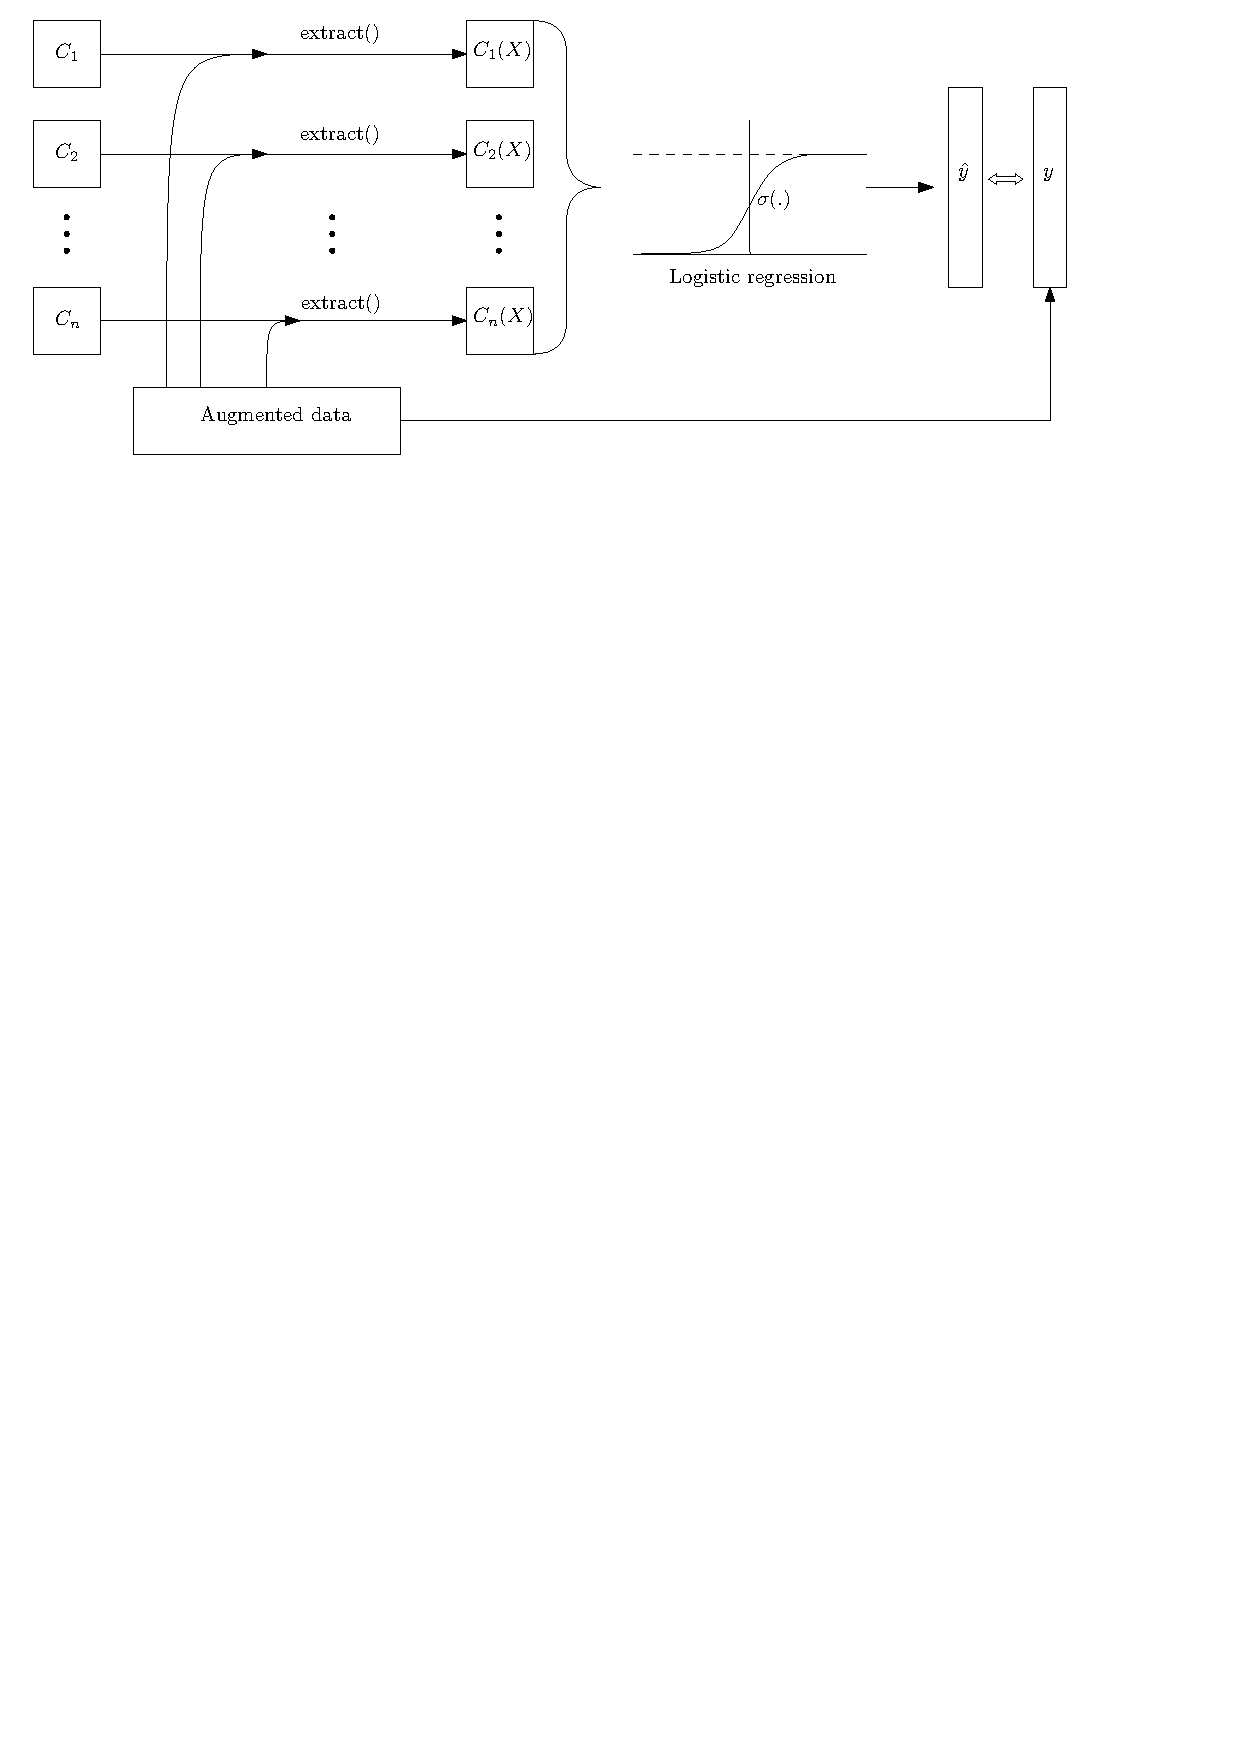
\includegraphics[scale=0.8]{fig/logistic_fitting.pdf}
		\caption{Main components of the global approach.}
		\label{Main}
	\end{figure}

The core components of our approach can be seen in figure \ref*{Main}. As described in section 2, the $C_i$ are the feature extractors and indicates a mapping:
\begin{equation}
C: \mathbb{S}^5 \rightarrow \mathbb{R}^l
\end{equation}
That is, it's a function of the set of all 5 sentence stories ($\mathbb{S}^5$) to a real vector.

%The math/architecture of your model. This should formally describe your idea from above. If you really want to, you can merge the two sections.

\section{Training}
What is your objective? How do you optimize it?

\section{Experiments}
This {\bf must} at least include the accuracy of your method on the validation set.
\section{Conclusion}
You can keep this short, too. \cite{*}

\bibliographystyle{plain}
\bibliography{bib/bib}
\end{document}
